\documentclass[final]{siamltex}

\usepackage{color}

% some extra math symbols
\usepackage{mathtools}

% for bold \mathcal font
\usepackage{bm}

% for figure environment
\usepackage{epsfig}

\setlength{\marginparwidth}{0.75in}
\newcommand{\MarginPar}[1]{\marginpar{\vskip-\baselineskip\raggedright\tiny\sffamily\hrule\smallskip{\color{red}#1}\par\smallskip\hrule}}

% for non-stacked fractions
\newcommand{\sfrac}[2]{\mathchoice
  {\kern0em\raise.5ex\hbox{\the\scriptfont0 #1}\kern-.15em/
   \kern-.15em\lower.25ex\hbox{\the\scriptfont0 #2}}
  {\kern0em\raise.5ex\hbox{\the\scriptfont0 #1}\kern-.15em/
   \kern-.15em\lower.25ex\hbox{\the\scriptfont0 #2}}
  {\kern0em\raise.5ex\hbox{\the\scriptscriptfont0 #1}\kern-.2em/
   \kern-.15em\lower.25ex\hbox{\the\scriptscriptfont0 #2}}
  {#1\!/#2}}

\renewcommand{\topfraction}{0.9}
\renewcommand{\bottomfraction}{0.9}
\renewcommand{\textfraction}{0.2}

\def\Fb {{\bf F}}
\def\gb {{\bf g}}
\def\mb {{\bf m}}
\def\Ub {{\bf U}}

\def\bA {\bm{\mathcal{A}}}
\def\bB {\bm{\mathcal{B}}}
\def\bI {\bm{\mathcal{I}}}
\def\bR {\bm{\mathcal{R}}}

\def\taub {\boldsymbol{\tau}}
\def\psib {\boldsymbol{\psi}}

\def\half   {\frac{1}{2}}
\def\myhalf {\sfrac{1}{2}}

\begin{document}

%==========================================================================
% Title
%==========================================================================
\title{Low Mach Number Stochastic Mixing Model Using Staggered Grids}

\maketitle

%==========================================================================
% Abstract and Keywords
%==========================================================================
\begin{abstract}
Abstract
\end{abstract}

\begin{keywords}
(Keywords)
\end{keywords}

\begin{AMS}
(AMR Classification Numbers)
\end{AMS}

%==========================================================================
% Introduction
%==========================================================================
\section{Introduction}


%==========================================================================
% Equations
%==========================================================================
\section{Equations}
We have two incompressible fluids with densities $\bar\rho_1$ and $\bar\rho_2$, where each fluid does not 
change volume upon mixing.  Defining $\rho$ to be the density of a mixture of these fluids, the densities of
each fluid are $\rho_1 \equiv \rho c$ and $\rho_2 \equiv \rho(1-c)$, where $c$ is the {\it mass} fraction of the 
first fluid.  Thus, $\rho = \rho_1 + \rho_2$.  Since the fluids do not change volume upon mixing, the equation 
of state will enforce that the {\it volume} fractions must sum to 1:
\begin{equation}
\frac{\rho_1}{\bar\rho_1} + \frac{\rho_2}{\bar\rho_2} =
\frac{\rho c}{\bar\rho_1} + \frac{\rho(1-c)}{\bar\rho_2} = 1 
\quad \rightarrow \quad
\rho = \left(\frac{c}{\bar\rho_1} + \frac{1-c}{\bar\rho_2}\right)^{-1}.
\end{equation}
The isothermal low Mach number equations of motion are:
\begin{eqnarray}
\frac{\partial\rho}{\partial t} &=& -\nabla\cdot(\rho\Ub),\label{eq:rho}\\
\frac{\partial\rho_1}{\partial t} &=& -\nabla\cdot(\rho_1\Ub) + \nabla\cdot\rho\chi\nabla c + F_{\rho_1} + \nabla\cdot\bA,\label{eq:rho1}\\
\frac{\partial\mb}{\partial t} &=& -\nabla\cdot(\mb\Ub) - \nabla\pi + \nabla\cdot\taub + \rho\gb + \Fb_{\mb} + \nabla\cdot\bB,\label{eq:m}
\end{eqnarray}
where $\Ub=(u,v)$ is the velocity, $\mb=(m_x,m_y)$ is the momentum, $\pi$ is the dynamic pressure, $\chi$ is the 
diffusion coefficient, $\gb$ is the gravitational vector, $F_{\rho_1}$ and $\Fb_{\mb}$ are external body forces, $\bA$ and $\bB$ are appropriately weighted white-noise
random vector and tensor fields, respectively.  We are still settling on the exact form of $\bA$ and $\bB$,
and will provide more details soon.  It is very likely that $\bA$ and $\bB$ will be functions of 
$\eta$, $\chi$, $\rho$, and likely $c$.  Here, $\taub$ is the stress tensor,
\begin{equation}
\taub = \eta\left[\nabla\Ub + (\nabla\Ub)^T\right] + \bI\left(\kappa-\frac{2}{3}\eta\right)(\nabla\cdot\Ub),\label{eq:stress tensor}
\end{equation}
where $\eta$ is the viscosity, $\kappa$ is the bulk velocity and $\bI$ is the identity tensor.
To derive a contraint on the velocity field, we begin by differentiating the equation of state, $\rho=\rho(\rho_1)$,
along particle paths,
\begin{equation}
\frac{D\rho}{Dt} = \frac{\partial\rho}{\partial\rho_1}\frac{D\rho_1}{Dt}.\label{eq:constraint 1}
\end{equation}
From the equations of motion:
\begin{equation}
\frac{D\rho}{Dt} = -\rho\nabla\cdot\Ub,\label{eq:constraint 2}
\end{equation}
\begin{equation}
\rho\frac{Dc}{Dt} = \underbrace{\nabla\cdot\rho\chi\nabla c + F_{\rho_1} + \nabla\cdot\bA}_{\widetilde S}.\label{eq:constraint 3}
\end{equation}
The equation of state can be arranged as:
\begin{equation}
\frac{\rho_1}{\bar\rho_1} + \frac{\rho_2}{\bar\rho_2} =
\frac{\rho_1}{\bar\rho_1} + \frac{(\rho-\rho_1)}{\bar\rho_2} = 1
\quad \rightarrow \quad
\rho = \bar\rho_2 - \rho_1\bar\rho_2\left(\frac{1}{\bar\rho_1} - \frac{1}{\bar\rho_2}\right),
\end{equation}
so that the partial derivative follows directly,
\begin{equation}
\frac{\partial\rho}{\partial\rho_1} = -\bar\rho_2\left(\frac{1}{\bar\rho_1} - \frac{1}{\bar\rho_2}\right).\label{eq:constraint 4}
\end{equation}
Plugging (\ref{eq:constraint 2}), (\ref{eq:constraint 3}), and (\ref{eq:constraint 4}), into (\ref{eq:constraint 1}) and
rearranging terms gives
\begin{equation}
\nabla\cdot\Ub = \left(\frac{1}{\bar\rho_1}-\frac{1}{\bar\rho_2}\right)\widetilde S \equiv S.
\end{equation}

%==========================================================================
% Equations
%==========================================================================
\section{Implementation}
Our numerical strategy is a conserative finite-volume approach.  We define 
the densities, $\rho$ and $\rho_1$, and the thermodynamic coefficients, 
$\chi, \eta$, and $\kappa$, on a regular Cartesian grid.
We also define momentum on a regular Cartesian grid, but we stagger the momentum such that 
the $i^{\rm th}$ component of momentum is centered about the faces of the 
Cartesian grid that defines the densities in the $i^{\rm th}$ direction
(see Figure \ref{fig:grid}).  In this paper, the terms ``cell-centered''
and ``face-centered'' refer to spatial locations in the reference frame
of the densities.  Also, a quantity with subscript ``$i,j$'' refers to a cell-based
quantity, whereas a half integer subscript, e.g., ``$i+\myhalf,j$''
refers to an face quantity.
%%%%%%%%%%%%%%%%%%%%%%%%%%%%%%%%%
\begin{figure}[tb]
\centering
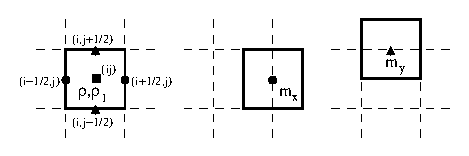
\includegraphics[width=6in]{grid}
\label{fig:grid}
\caption{Cartesian grid, finite volume grid structure with ``cell-centered'' densities
and staggered momenta.}
\end{figure}
%%%%%%%%%%%%%%%%%%%%%%%%%%%%%%%%%

Our spatial discretizations are second order, but we can achieve arbitrary temporal order of
accuracy by using an explicit multi-stage integration strategy.  Given an input 
state $(\rho,\rho_1,\mb)^{\rm in}$, we define a stage evaluation as a projection
of the velocities onto the $\nabla\cdot\Ub=S$ constraint followed by the the 
computation of remaining terms in the
right-hand-side of equations (\ref{eq:rho}), (\ref{eq:rho1}), and (\ref{eq:m}) (the
$\nabla\pi$ term is accounted for in the projection).
We use the notation
$\mathcal{F}^{\rm in} \equiv \mathcal{F}(\phi^{\rm in},S(\phi^{\rm in}))$ 
to denote the evaluation of these remaining terms.  An
example of a simple temporal integration is a second-order midpoint corrector, which 
requires two stage evaluations:
\begin{eqnarray}
\phi^{(1)} &=& \phi^n + \frac{\Delta t}{2}\mathcal{F}^n,\\
\phi^{n+1} &=& \phi^n + \Delta t\mathcal{F}^{(1)}.
\end{eqnarray}
Another option is a second-order trapezoidal corrector:
\begin{eqnarray}
\phi^{(1)} &=& \phi^n + \Delta t\mathcal{F}^n,\\
\phi^{n+1} &=& \frac{\phi^n + \phi^{(1)}}{2} + \frac{\Delta t}{2}\mathcal{F}^{(1)}\nonumber\\
&=& \phi^n + \Delta t\left(\frac{\mathcal{F}^n+\mathcal{F}^{(1)}}{2}\right)
\end{eqnarray}
Another option is a two-stage RK3 scheme:
\begin{eqnarray}
\phi^{(1)} &=& \phi^n + \Delta t\mathcal{F}^n,\\
\phi^{(2)} &=& \frac{3}{4}\phi^n + \frac{1}{4}\left[\phi^{(1)} + \Delta t\mathcal{F}^{(1)}\right],\\
\phi^{n+1} &=& \frac{1}{3}\phi^n + \frac{2}{3}\left[\phi^{(2)} + \Delta t\mathcal{F}^{(2)}\right].
\end{eqnarray}
In order to satisfy the equation of state, the discretization of the advection terms
in a stage evaluation must use velocities that discretely satifsy the divergence constraint.
In doing so, we are guaranteed to stay on the equation of state up to solver tolerance.

\subsection{Stage Evaluation Discretization}
The stage evaluation is an explicit process given input $\phi^{\rm in}$.  Here is how we 
define the stage evaluations, given an input state $(\rho,\rho_1,\mb)$.\\

\begin{itemize}

\item {\bf Step 1}: {\it Compute stochastic terms, $\nabla\cdot\bA$ and $\nabla\cdot\bB$}.\\

Details coming soon!\\

\item {\bf Step 2}: {\it Compute diffusive terms, $\nabla\cdot\rho\chi\nabla c$}.\\

We evalute $\nabla\cdot\rho\chi\nabla c$ at cell-centers using the discretization:
\begin{equation}
(\nabla\cdot\rho\chi\nabla c)_{i,j} = \frac{\left(\rho\chi \frac{\partial c}{\partial x}\right)_{i+\myhalf,j} - \left(\rho\chi \frac{\partial c}{\partial x}\right)_{i-\myhalf,j}}{\Delta x}
+ \frac{\left(\rho\chi \frac{\partial c}{\partial y}\right)_{i,j+\myhalf} - \left(\rho\chi \frac{\partial c}{\partial y}\right)_{i,j-\myhalf}}{\Delta y},
\end{equation}
where, e.g.,
\begin{eqnarray}
\left(\rho\chi \frac{\partial c}{\partial x}\right)_{i+\myhalf,j} &=& \left(\rho_{i+\myhalf,j}\right)\left(\chi_{i+\myhalf,j}\right)\left(\frac{c_{i+1,j}-c_{i,j}}{\Delta x}\right),\\
\left(\rho\chi \frac{\partial c}{\partial y}\right)_{i,j+\myhalf} &=& \left(\rho_{i,j+\myhalf}\right)\left(\chi_{i,j+\myhalf}\right)\left(\frac{c_{i,j+1}-c_{i,j}}{\Delta y}\right),
\end{eqnarray}
with, e.g.,
\begin{equation}
\rho_{i+\myhalf,j} = \frac{\rho_{i,j}+\rho_{i+1,j}}{2}, \quad \chi_{i+\myhalf,j} = \frac{\chi_{i,j}+\chi_{i+1,j}}{2},
\end{equation}
and $c_{i,j} = (\rho_1)_{i,j}/\rho_{i,j}$.\\

\item {\bf Step 3}: {\it Compute the projected velocity field, $\Ub^{\rm MAC}$}.\\

First, compute unprojected velocities ($u^*$ on $x$-faces and $v^*$ on $y$-faces) from 
$\Ub$, $\rho$, and $\mb$, using simple averaging, e.g.,
\begin{equation}
u_{i+\myhalf,j}^* = \frac{(m_x)_{i+\myhalf,j}}{\rho_{i+\myhalf,j}}, \qquad
v_{i,j+\myhalf}^* = \frac{(m_y)_{i,j+\myhalf}}{\rho_{i,j+\myhalf}}.
\end{equation}
Then, solve an elliptic equation for cell-centered $\phi$,
\begin{equation}
\nabla\cdot\frac{1}{\rho}\nabla\phi = \nabla\cdot\Ub^* - S,
\end{equation}
using
\begin{eqnarray}
\frac{1}{\Delta x}\left[\left(\frac{1}{\rho_{i+\myhalf,j}}\right)\left(\frac{\phi_{i+1,j}-\phi_{i,j}}{\Delta x}\right) - \left(\frac{1}{\rho_{i-\myhalf,j}}\right)\left(\frac{\phi_{i,j}-\phi_{i,j-1}}{\Delta x}\right)\right]&&\nonumber\\
+ \frac{1}{\Delta y}\left[\left(\frac{1}{\rho_{i,j+\myhalf}}\right)\left(\frac{\phi_{i,j+1}-\phi_{i,j}}{\Delta y}\right) - \left(\frac{1}{\rho_{i,j-\myhalf}}\right)\left(\frac{\phi_{i,j}-\phi_{i,j-1}}{\Delta y}\right)\right]&&\nonumber\\
= S_{i,j} - \left[\left(\frac{u_{i+\myhalf,j}^*-u_{i-\myhalf,j}^*}{\Delta x}\right) + \left(\frac{v_{i,j+\myhalf}^*-v_{i,j-\myhalf}^*}{\Delta y}\right)\right].&&
\end{eqnarray}
Next, compute the MAC velocities,
\begin{equation}
\Ub^{\rm MAC} = \Ub^* - \frac{1}{\rho}\nabla\phi,
\end{equation}
using, e.g.,
\begin{equation}
u^{\rm MAC}_{i+\myhalf,j} = u_{i+\myhalf,j}^* - \frac{1}{\rho_{i+\myhalf,j}}\left(\frac{\phi_{i+1,j}-\phi_{i,j}}{\Delta x}\right).
\end{equation}

\item {\bf Step 4}: {\it Compute advection terms, $\nabla\cdot(\rho\Ub)$, $\nabla\cdot(\rho_1\Ub)$, and $\nabla\cdot(\mb\Ub)$}.\\

For $\rho$ and $\rho_1$, we first average the density to faces, and then use a standard flux 
divergence stencil, e.g.,
\begin{equation}
\nabla\cdot(\rho\Ub) = \frac{\rho_{i+\myhalf,j}^{\rm in}u_{i+\myhalf,j}^{\rm MAC} - \rho_{i-\myhalf,j}^{\rm in}u_{i-\myhalf,j}^{\rm MAC}}{\Delta x} + \frac{\rho_{i,j+\myhalf}^{\rm in}v_{i,j+\myhalf}^{\rm MAC} - \rho_{i,j-\myhalf}^{\rm in}v_{i,j-\myhalf}^{\rm MAC}}{\Delta y}.
\end{equation}
The advection terms for momentum are a bit more complicated (index-wise) since they live on a staggered grid.
The fluxes corresponding to the momentum centered at $(i+\myhalf,j)$ are located at $(ij)$ and 
$(i+1,j)$ (the $x$-fluxes) and $(i+\myhalf,j-\myhalf)$ and $(i+\myhalf,j+\myhalf)$ (the $y$-fluxes), e.g.,
\begin{equation}
\nabla\cdot(m_x\Ub)_{i+\myhalf,j} = \frac{(m_xu)_{i+1,j}-(m_xu)_{i,j}}{\Delta x} + \frac{(m_xv)_{i+\myhalf,j+\myhalf}-(m_xv)_{i+\myhalf,j-\myhalf}}{\Delta y},
\end{equation}
with
\begin{equation}
(m_x u)_{i,j} = \left(\frac{(m_x)_{i-\myhalf,j} + (m_x)_{i+\myhalf,j}}{2}\right)\left(\frac{u_{i-\myhalf,j}^{\rm MAC} + u_{i+\myhalf,j}^{\rm MAC}}{2}\right),
\end{equation}
\begin{equation}
(m_x v)_{i+\myhalf,j+\myhalf} = \left(\frac{(m_x)_{i+\myhalf,j}+(m_x)_{i+\myhalf,j+1}}{2}\right)\left(\frac{v_{i,j+\myhalf}^{\rm MAC}+v_{i+1,j+\myhalf}^{\rm MAC}}{2}\right).
\end{equation}
Note that the velocity field represented by $u^{\rm MAC}$ averaged to cell-centers and 
$v^{\rm MAC}$ averaged to nodes also satisfies a form of the divergence constraint with 
$S$ averaged to faces.\\

\item {\bf Step 5}: {\it Compute viscous terms, $\nabla\cdot\taub$}.\\

In our simplified model, $\nabla\cdot\taub = \nabla\cdot\eta[\nabla\Ub+(\nabla\Ub)^T]$.
\begin{equation}
\nabla\cdot\taub
=
\left[\begin{array}{c}
2\frac{\partial}{\partial x}\left(\eta\frac{\partial u}{\partial x}\right) + \frac{\partial}{\partial y}\left[\eta\frac{\partial u}{\partial y} + \eta\frac{\partial v}{\partial x}\right]\\
2\frac{\partial}{\partial y}\left(\eta\frac{\partial v}{\partial y}\right) + \frac{\partial}{\partial x}\left[\eta\frac{\partial v}{\partial x} + \eta\frac{\partial u}{\partial y}\right]
\end{array}\right].
\end{equation}
The discretization of this viscous terms requires $\eta$ at cell-centers and nodes.  The value of $\eta$ at a node is simply the average of the four neighboring cell-centers.
Term by term, the discretization of $\nabla\cdot\taub$ for the $x$-component of momentum:
\begin{equation}
\left[\frac{\partial}{\partial x}\left(\eta\frac{\partial u}{\partial x}\right)\right]_{i+\myhalf,j} = \frac{(\eta \frac{\partial u}{\partial x})_{i+1,j}-(\eta \frac{\partial u}{\partial x})_{i,j}}{\Delta x}
\end{equation}
with
\begin{equation}
\left(\eta \frac{\partial u}{\partial x}\right)_{i,j} = \eta_{i,j}\left(\frac{u_{i+\myhalf,j}^{\rm MAC} - u_{i-\myhalf,j}^{\rm MAC}}{\Delta x}\right),
\end{equation}
\begin{equation}
\left[\frac{\partial}{\partial y}\left(\eta\frac{\partial u}{\partial y}\right)\right]_{i+\myhalf,j} = \frac{(\eta \frac{\partial u}{\partial y})_{i+\myhalf,j+\myhalf} - (\eta\frac{\partial u}{\partial y})_{i+\myhalf,j-\myhalf}}{\Delta y},
\end{equation}
with
\begin{equation}
\left(\eta \frac{\partial u}{\partial y}\right)_{i+\myhalf,j+\myhalf} = \eta_{i+\myhalf,j+\myhalf}\left(\frac{u_{i+\myhalf,j+1}^{\rm MAC} - u_{i+\myhalf,j}^{\rm MAC}}{\Delta y}\right),
\end{equation}
\begin{equation}
\left[\frac{\partial}{\partial y}\left(\eta\frac{\partial v}{\partial x}\right)\right]_{i+\myhalf,j} = \frac{(\eta \frac{\partial v}{\partial x})_{i+\myhalf,j+\myhalf} - (\eta\frac{\partial v}{\partial x})_{i+\myhalf,j-\myhalf}}{\Delta y},
\end{equation}
with
\begin{equation}
\left(\eta \frac{\partial v}{\partial x}\right)_{i+\myhalf,j+\myhalf} = \eta_{i+\myhalf,j+\myhalf}\left(\frac{v_{i+1,j+\myhalf}^{\rm MAC} - v_{i,j+\myhalf}^{\rm MAC}}{\Delta x}\right).
\end{equation}

\item {\bf Step 6}: {\it Compute gravitational and external body forces}.\\

We compute $\rho\gb$, $F_{\rho_1}$, and $\Fb_{\mb}$ as functions of $\rho^{\rm in}$ and $\rho_1^{\rm in}$.\\

\end{itemize}
At this point we have all the terms required for the stage evaluation.  Note once the temporal 
advancement is complete and the state at $t^{n+1}$ has been computed, we perform 
{\bf Steps 1-3} to ensure that the final velocity field satisfies the divergence constraint.
This also implies that a stage evaluation that uses the state at $t^n$ as the input state 
can skip {\bf Steps 1-3}, since the velocity field has already been projected and the terms 
in the divergence constraint have already been computed.

\subsection{Boundary Conditions}
In our code, we use two rows of ghost cells for cell-centered data, and one row of ghost cells for staggered data
(see Figure \ref{fig:ghost}).  The periodic case is straightforward so we focus on the non-periodic cases here.
We currently have three different types of non-periodic boundary conditions: 
{\tt SLIP\_WALL}, {\tt NO\_SLIP\_WALL}, and {\tt INLET}.  We define ``normal'' and ``transverse'' 
velocities with respect to the direction of the boundary face we are interested in.
Our numerical implementation for ghost cells differs for 
normal staggered velocity, transverse staggered velocities, and cell-centered scalars ($\rho$ and $c$).
Our physical interpretation is as follows:
\begin{itemize}
\item {\tt SLIP\_WALL}:
\begin{itemize}
\item Normal velocity: homogeneous Dirichlet 
\item Transverse velocities: homogeneous Neumann
\item Scalars: homogeneous Neumann
\end{itemize}
\item {\tt NO\_SLIP\_WALL}:
\begin{itemize}
\item Normal velocity: homogeneous Dirichlet 
\item Transverse velocities: prescribed Dirichlet
\item Scalars: homogeneous Neumann
\end{itemize}
\item {\tt INLET}:
\begin{itemize}
\item Normal velocity: prescribed Dirichlet 
\item Transverse velocities: prescribed Dirichlet
\item Scalars: prescribed Dirichlet
\end{itemize}
\end{itemize}
%%%%%%%%%%%%%%%%%%%%%%%%%%%%%%%%%
\begin{figure}[tb]
\centering
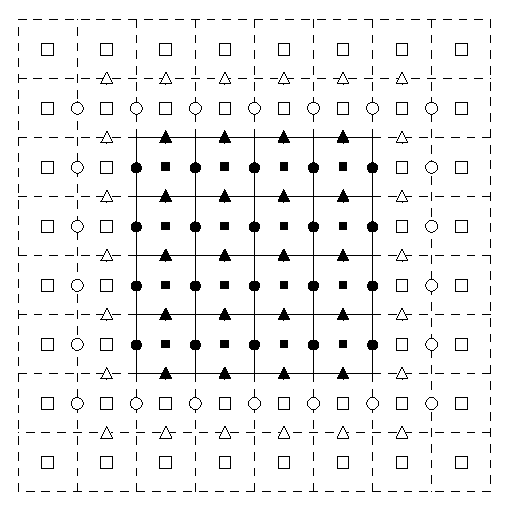
\includegraphics[width=3in]{ghost}
\label{fig:ghost}
\caption{A sample 4$\times$4 grid with two rows of ghost cells for cell-centered data and one row of
ghost cells for staggered data.  Valid cell-centered data are centered about the dark squares whereas the 
ghost cells are centered about the open squares.  The valid $x$ and $y$-staggered grid data are centered 
about the dark circles and triangles, whereas the ghost data is centered about the open circles and triangles.}
\end{figure}
%%%%%%%%%%%%%%%%%%%%%%%%%%%%%%%%%
We now describe the implementation details.

\subsubsection{Scalars}
The subroutine {\tt multifab\_physbc} fills in ghost cells for $\rho$ and $c$.
The guiding principle shall be that ghost cells values refer to {\it the value at the boundary}.
For Dirichlet conditions, the ghost cells contains the prescribed Dirichlet value.
For a homogeneous Neumann condition, we set the ghost cell values equal to the interior value.
Transport coefficients, which are functions of $\rho$ and $c$, are always evaluated at cell-centers 
and later averaged to faces and/or nodes.  However, at faces and nodes that lie on physical 
boundaries, we evaluate transport coefficients directly from the boundary state.

\subsubsection{Transverse Velocities}
The subroutine {\tt multifab\_physbc\_macvel} fills in ghost cells for the transverse velocities.
The guiding principle shall be that ghost cells {\tt behind} physical boundaries refer to 
{\it an extrapolated value}.  For a Dirichlet conditions, the ghost cells contain a value linearly
extrapolated from the interior cell and the prescribed Dirichlet value.
For a homogeneous Neumann condition, we set the ghost cell values equal to the interior value.  

\subsubsection{Normal Velocity}

Normal velocity is a unique case in that values lie on physical boundaries.
The guiding principle shall be that ghost cells 
{\it on and behind} physical boundaries refer to {\it the value at the boundary}.
The subroutine {\tt multifab\_physbc\_domainvel} sets the value on the boundary to the Dirichlet
value, where the subroutine {\tt multifab\_physbc\_macvel} sets the ghost cells to the value
on the boundary.  The reason we have two subroutines is that sometimes we must externally modify
the normal velocity on the domain boundary.  An example of this is when we have a diffusive flux
of scalars entering at an inflow boundary condition and the velocity on the domain boundary must
be altered so that we stay on the EOS.  In that case, we may not want to call
{\tt multifab\_physbc\_domainvel} to overwrite the normal velocity, but may need to call
{\tt multifab\_physbc\_macvel} to update the ghost cells.

\section{Viscous Operators}
Recall that the divergence of the full viscous stress tensor is
\begin{equation}
\mathcal{D}\Ub = \nabla\cdot\left\{\eta\left[\nabla\Ub + (\nabla\Ub)^T\right] + \bI\left(\kappa-\frac{2}{3}\eta\right)(\nabla\cdot\Ub)\right\}.
\end{equation}
We enable this formulation with {\tt viscous\_type}=-3.  A negative value of {\tt viscous\_type} means 
that we implement a stress tensor with spatially varying $\eta$ and $\kappa$.  A positive value of 
{\tt viscous\_type} means that $\eta$ and $\kappa$ are constant in space, and have more efficient
and compact stencils in the code.  A slightly simpler model that assumes $\kappa = \frac{2}{3}\eta$ 
({\tt viscous\_type}=-2) is
\begin{equation}
\mathcal{D}\Ub = \nabla\cdot\left\{\eta\left[\nabla\Ub + (\nabla\Ub)^T\right]\right\}.
\end{equation}
An even simpler model ({\tt viscous\_type}=-1) is
\begin{equation}
\mathcal{D}\Ub = \nabla\cdot\eta\nabla\Ub.
\end{equation}
In Figures \ref{fig:viscOp} and \ref{fig:viscOp_3d}, we illustrate the 2D and 3D stencils for 
the $x$-component of each term in the full viscous stress tensor.
The black circles indicate locations of $u$,.
The black triangles indicate locations of $v$ (and $w$).
The red dots indicate the location of the $\beta$ and the gradients of velocity.  
Note that in 2D we require $\beta$ at nodes, whereas in 3D we require $\beta$ at edges.
%%%%%%%%%%%%%%%%%%%%%%%%%%%%%%%%%
\begin{figure}[tb]
\centering
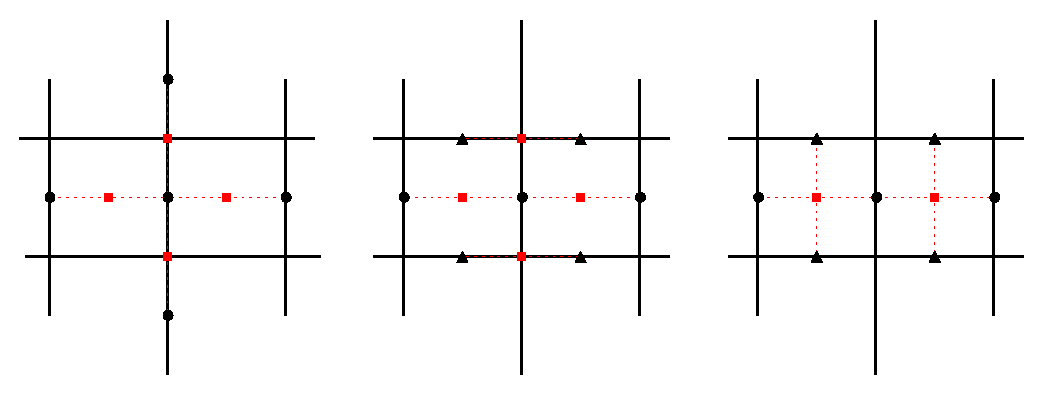
\includegraphics[width=5.25in]{viscOp}
\label{fig:viscOp}
\caption{The stencils for the $x$-component of (Left) $\nabla\cdot\eta\nabla\Ub$, (Middle) 
$\nabla\cdot\eta(\nabla\Ub)^T$, and (Right) $\nabla\cdot[\bI(\kappa-\frac{2}{3}\eta)(\nabla\cdot\Ub)]$.  
The black circles indicate locations of $u$.
The black triangles indicate locations of $v$.
The red dots indicate the location of the $\beta$ and the gradients of velocity.}
\end{figure}
%%%%%%%%%%%%%%%%%%%%%%%%%%%%%%%%%
%%%%%%%%%%%%%%%%%%%%%%%%%%%%%%%%%
\begin{figure}[tb]
\centering
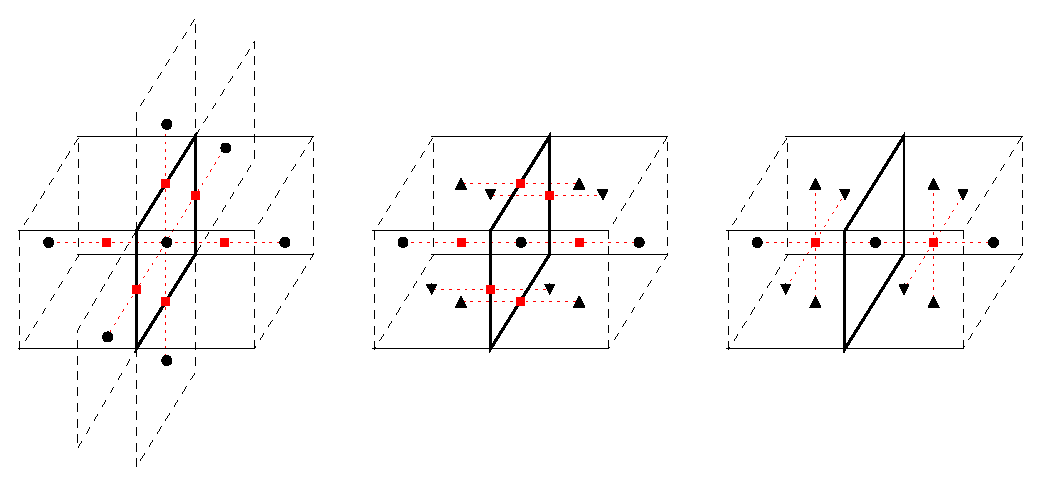
\includegraphics[width=5.25in]{viscOp_3d}
\label{fig:viscOp_3d}
\caption{The stencils for the $x$-component of (Left) $\nabla\cdot\eta\nabla\Ub$, (Middle) 
$\nabla\cdot\eta(\nabla\Ub)^T$, and (Right) $\nabla\cdot[\bI(\kappa-\frac{2}{3}\eta)(\nabla\cdot\Ub)]$.  
The black circles indicate locations of $u$.
The black triangles indicate locations of $v$ and $w$.
The red dots indicate the location of the $\beta$ and the gradients of velocity.}
\end{figure}
%%%%%%%%%%%%%%%%%%%%%%%%%%%%%%%%%

Term by term,
\begin{equation}
\nabla\cdot\eta\nabla\Ub = \frac{\partial}{\partial x_j}\left(\eta\frac{\partial u_i}{\partial x_j}\right) =
\left[\begin{array}{c}
\frac{\partial}{\partial x}\left(\eta\frac{\partial u}{\partial x}\right) + 
\frac{\partial}{\partial y}\left(\eta\frac{\partial u}{\partial y}\right) +
\frac{\partial}{\partial z}\left(\eta\frac{\partial u}{\partial z}\right)\\
\frac{\partial}{\partial x}\left(\eta\frac{\partial v}{\partial x}\right) + 
\frac{\partial}{\partial y}\left(\eta\frac{\partial v}{\partial y}\right) +
\frac{\partial}{\partial z}\left(\eta\frac{\partial v}{\partial z}\right)\\
\frac{\partial}{\partial x}\left(\eta\frac{\partial w}{\partial x}\right) + 
\frac{\partial}{\partial y}\left(\eta\frac{\partial w}{\partial y}\right) +
\frac{\partial}{\partial z}\left(\eta\frac{\partial w}{\partial z}\right)
\end{array}\right]
\end{equation}
\begin{equation}
\nabla\cdot\eta(\nabla\Ub)^T = \frac{\partial}{\partial x_j}\left(\eta\frac{\partial u_j}{\partial x_i}\right) =
\left[\begin{array}{c}
\frac{\partial}{\partial x}\left(\eta\frac{\partial u}{\partial x}\right) + 
\frac{\partial}{\partial y}\left(\eta\frac{\partial v}{\partial x}\right) +
\frac{\partial}{\partial z}\left(\eta\frac{\partial w}{\partial x}\right)\\
\frac{\partial}{\partial x}\left(\eta\frac{\partial u}{\partial y}\right) + 
\frac{\partial}{\partial y}\left(\eta\frac{\partial v}{\partial y}\right) +
\frac{\partial}{\partial z}\left(\eta\frac{\partial w}{\partial y}\right)\\
\frac{\partial}{\partial x}\left(\eta\frac{\partial u}{\partial z}\right) + 
\frac{\partial}{\partial y}\left(\eta\frac{\partial v}{\partial z}\right) +
\frac{\partial}{\partial z}\left(\eta\frac{\partial w}{\partial z}\right)
\end{array}\right]
\end{equation}
\begin{equation}
\nabla\cdot\left[\bI\left(\kappa-\frac{2}{3}\eta\right)(\nabla\cdot\Ub)\right] = \frac{\partial}{\partial x_j}\left[\left(\kappa - \frac{2}{3}\eta\right)\frac{\partial u_k}{\partial x_k}\delta_{ji}\right] =
\left[\begin{array}{c}
\frac{\partial}{\partial x}\left[\left(\kappa-\frac{2}{3}\eta\right)\left(\frac{\partial u}{\partial x} + \frac{\partial v}{\partial y} + \frac{\partial w}{\partial x}\right)\right]\\
\frac{\partial}{\partial y}\left[\left(\kappa-\frac{2}{3}\eta\right)\left(\frac{\partial u}{\partial x} + \frac{\partial v}{\partial y} + \frac{\partial w}{\partial x}\right)\right]\\
\frac{\partial}{\partial z}\left[\left(\kappa-\frac{2}{3}\eta\right)\left(\frac{\partial u}{\partial x} + \frac{\partial v}{\partial y} + \frac{\partial w}{\partial x}\right)\right]
\end{array}\right]
\end{equation}

For the $x$-component in 2D:
\begin{eqnarray}
\nabla\cdot\eta\nabla\Ub = \frac{\partial}{\partial x_j}\left(\eta\frac{\partial u_i}{\partial x_j}\right) &\rightarrow&
\frac{\partial}{\partial x}\left(\eta\frac{\partial u}{\partial x}\right) + 
\frac{\partial}{\partial y}\left(\eta\frac{\partial u}{\partial y}\right)\nonumber\\
&=& \left(\frac{-\eta_{i+1,j} - \eta_{i,j} - \eta_{i+\myhalf,j+\myhalf} - \eta_{i+\myhalf,j-\myhalf}}{h^2}\right)u_{i+\myhalf,j}\nonumber\\
&& + \left(\frac{\eta_{i+1,j}}{h^2}\right)u_{i+\sfrac{3}{2},j}\nonumber\\
&& + \left(\frac{\eta_{i,j}}{h^2}\right)u_{i-\myhalf}\nonumber\\
&& + \left(\frac{\eta_{i+\myhalf,j+\myhalf}}{h^2}\right)u_{i+\myhalf,j+1}\nonumber\\
&& + \left(\frac{\eta_{i+\myhalf,j-\myhalf}}{h^2}\right)u_{i+\myhalf,j-1},\label{eq:visc1}
\end{eqnarray}
\begin{eqnarray}
\nabla\cdot\eta(\nabla\Ub)^T = \frac{\partial}{\partial x_j}\left(\eta\frac{\partial u_j}{\partial x_i}\right) &\rightarrow&
\frac{\partial}{\partial x}\left(\eta\frac{\partial u}{\partial x}\right) + 
\frac{\partial}{\partial y}\left(\eta\frac{\partial v}{\partial x}\right)\nonumber\\
&=& \left(\frac{-\eta_{i+1,j} - \eta_{i,j}}{h^2}\right)u_{i+\myhalf,j}\nonumber\\
&& + \left(\frac{\eta_{i+1,j}}{h^2}\right)u_{i+\sfrac{3}{2},j}\nonumber\\
&& + \left(\frac{\eta_{i,j}}{h^2}\right)u_{i-\myhalf,j}\nonumber\\
&& + \left(\frac{\eta_{i+\myhalf,j+\myhalf}}{h^2}\right)v_{i+1,j+\myhalf}\nonumber\\
&& + \left(-\frac{\eta_{i+\myhalf,j+\myhalf}}{h^2}\right)v_{i,j+\myhalf}\nonumber\\
&& + \left(-\frac{\eta_{i+\myhalf,j-\myhalf}}{h^2}\right)v_{i+1,j-\myhalf}\nonumber\\
&& + \left(\frac{\eta_{i+\myhalf,j-\myhalf}}{h^2}\right)v_{i,j-\myhalf},
\end{eqnarray}
\begin{eqnarray}
\nabla\cdot\left[\bI\left(\kappa-\frac{2}{3}\eta\right)(\nabla\cdot\Ub)\right] = \frac{\partial}{\partial x_j}\left[\left(\kappa - \frac{2}{3}\eta\right)\frac{\partial u_k}{\partial x_k}\delta_{ji}\right] &\rightarrow& 
\frac{\partial}{\partial x}\left[\left(\kappa-\frac{2}{3}\eta\right)\left(\frac{\partial u}{\partial x} + \frac{\partial v}{\partial y}\right)\right]\nonumber\\
&=& \left[\frac{-\left(\kappa-\frac{2}{3}\eta\right)_{i+1,j} - \left(\kappa-\frac{2}{3}\eta\right)_{i,j}}{h^2}\right]u_{i+\myhalf,j}\nonumber\\
&& + \left[\frac{\left(\kappa-\frac{2}{3}\eta\right)_{i+1,j}}{h^2}\right]u_{i+\sfrac{3}{2},j}\nonumber\\
&& + \left[\frac{\left(\kappa-\frac{2}{3}\eta\right)_{i,j}}{h^2}\right]u_{i-\myhalf,j}\nonumber\\
&& + \left[\frac{\left(\kappa-\frac{2}{3}\eta\right)_{i+1,j}}{h^2}\right]v_{i+1,j+\myhalf}\nonumber\\
&& + \left[\frac{-\left(\kappa-\frac{2}{3}\eta\right)_{i+1,j}}{h^2}\right]v_{i+1,j-\myhalf}\nonumber\\
&& + \left[\frac{-\left(\kappa-\frac{2}{3}\eta\right)_{i,j}}{h^2}\right]v_{i,j+\myhalf}\nonumber\\
&& + \left[\frac{\left(\kappa-\frac{2}{3}\eta\right)_{i,j}}{h^2}\right]v_{i,j-\myhalf}.
\end{eqnarray}
Collecting terms, the divergence of the stress tensor ({\tt viscous\_type}=-3) is:
\begin{eqnarray}
\mathcal{D}\Ub &=& 
\left(\frac{-\frac{4}{3}\eta_{i+1,j} - \kappa_{i+1,j} - \frac{4}{3}\eta_{i,j} - \kappa_{i,j} - \eta_{i+\myhalf,j+\myhalf} - \eta_{i+\myhalf,j-\myhalf}}{h^2}\right)u_{i+\myhalf,j}\nonumber\\
&& + \left(\frac{\frac{4}{3}\eta_{i+1,j} + \kappa_{i+1,j}}{h^2}\right)u_{i+\sfrac{3}{2},j}\nonumber\\
&& + \left(\frac{\frac{4}{3}\eta_{i,j} + \kappa_{i,j}}{h^2}\right)u_{i-\myhalf}\nonumber\\
&& + \left(\frac{\eta_{i+\myhalf,j+\myhalf}}{h^2}\right)u_{i+\myhalf,j+1}\nonumber\\
&& + \left(\frac{\eta_{i+\myhalf,j-\myhalf}}{h^2}\right)u_{i+\myhalf,j-1}\nonumber\\
&& + \left(\frac{\eta_{i+\myhalf,j+\myhalf} - \frac{2}{3}\eta_{i+1,j} + \kappa_{i+1,j}}{h^2}\right)v_{i+1,j+\myhalf}\nonumber\\
&& + \left(\frac{-\eta_{i+\myhalf,j+\myhalf} + \frac{2}{3}\eta_{i,j} - \kappa_{i,j}}{h^2}\right)v_{i,j+\myhalf}\nonumber\\
&& + \left(\frac{-\eta_{i+\myhalf,j-\myhalf} + \frac{2}{3}\eta_{i+1,j} - \kappa_{i+1,j}}{h^2}\right)v_{i+1,j-\myhalf}\nonumber\\
&& + \left(\frac{\eta_{i+\myhalf,j-\myhalf} - \frac{2}{3}\eta_{i,j} + \kappa_{i,j}}{h^2}\right)v_{i,j-\myhalf}.
\end{eqnarray}
For the simpler case ({\tt viscous\_type}=-2),
\begin{eqnarray}
\mathcal{D}\Ub &=& 
\left(\frac{-2\eta_{i+1,j} - 2\eta_{i,j} - \eta_{i+\myhalf,j+\myhalf} - \eta_{i+\myhalf,j-\myhalf}}{h^2}\right)u_{i+\myhalf,j}\nonumber\\
&& + \left(\frac{2\eta_{i+1,j}}{h^2}\right)u_{i+\sfrac{3}{2},j}\nonumber\\
&& + \left(\frac{2\eta_{i,j}}{h^2}\right)u_{i-\myhalf}\nonumber\\
&& + \left(\frac{\eta_{i+\myhalf,j+\myhalf}}{h^2}\right)u_{i+\myhalf,j+1}\nonumber\\
&& + \left(\frac{\eta_{i+\myhalf,j-\myhalf}}{h^2}\right)u_{i+\myhalf,j-1}\nonumber\\
&& + \left(\frac{\eta_{i+\myhalf,j+\myhalf}}{h^2}\right)v_{i+1,j+\myhalf}\nonumber\\
&& + \left(-\frac{\eta_{i+\myhalf,j+\myhalf}}{h^2}\right)v_{i,j+\myhalf}\nonumber\\
&& + \left(-\frac{\eta_{i+\myhalf,j-\myhalf}}{h^2}\right)v_{i+1,j-\myhalf}\nonumber\\
&& + \left(\frac{\eta_{i+\myhalf,j-\myhalf}}{h^2}\right)v_{i,j-\myhalf}.
\end{eqnarray}
For the simplest case ({\tt viscous\_type}=-1), the stencil is given in equation (\ref{eq:visc1}).

\section{Implicit Diffusion Notes}
Let's start by considering
\begin{equation}
\frac{\partial\mb}{\partial t} = \mathcal{D}\Ub.
\end{equation}
The backward-Euler discretization,
\begin{equation}
\frac{\mb^{n+1} - \mb^n}{\Delta t} = \mathcal{D}(\Ub^{n+1}),
\end{equation}
can be arranged into the following operator form:
\begin{equation}
\left(\rho^{n+1} - \Delta t\mathcal{D}\right)\Ub^{n+1} = \mb^n
\end{equation}
where $\Ub^{n+1}$ is the only unknown.  Thus, we seek to solve a system of the form:
\begin{equation}
\mathcal{L}\Ub \equiv \left\{\alpha - \nabla\cdot\left[\beta\left(\nabla+\nabla^T\right) + \bI\left(\gamma-\frac{2}{3}\beta\right)\nabla\cdot\right]\right\}\Ub = \bR,
\end{equation}
with $\alpha=\rho^{n+1}$, $\beta=\Delta t\cdot\eta$, $\gamma = \Delta t\cdot\kappa$,
and $\bR=\mb^n$.  We note that for {\tt |viscous\_type|}=1, there is no coupling between components, and we solve for each component of velocity individually.  Also, we note this is different from cell-centered multigrid in that $\Ub$ lives on a staggered grid.  Thus, we need $\alpha$ and $\beta$ at locations different from those in a standard cell-centered multigrid solver.  

\subsection{Multigrid Notes}
Functions we need for residual-correction multigrid.
\begin{itemize}
\item {\tt applyOp\_stag\_2d} and {\tt applyOp\_stag\_3d}\\
Computes $\mathcal{L}\psib$.  Here, we use $\psib$ to generally denote the velocity (at the finest level of multigrid), or the correction term (at coarser levels of multigrid).
\item Computing the residual:\\
Compute $\bR - \mathcal{L}\psib$
\item Performing a weighted Jacobi relaxation:\\
Updates $\psib^{k+1} = \psib^k + \omega D^{-1}[\bR - \mathcal{L}\psib^k]$, where $D$ is the diagonal elements of $\mathcal{L}$.
\item {\tt coarsen\_residual}\\
Coarsens $\bR - \mathcal{L}\psib$ and transfers it to the $\bR$ of the coarser level.
\item {\tt interpolate\_corection}\\
Interpolates $\psib$ to the finer level and corrects the finer $\psib$.
\end{itemize}

\end{document}
